\cleardoubleoddpage

\Scene{2}[Another part of the island.]

\begin{figure}[t!]
\centering
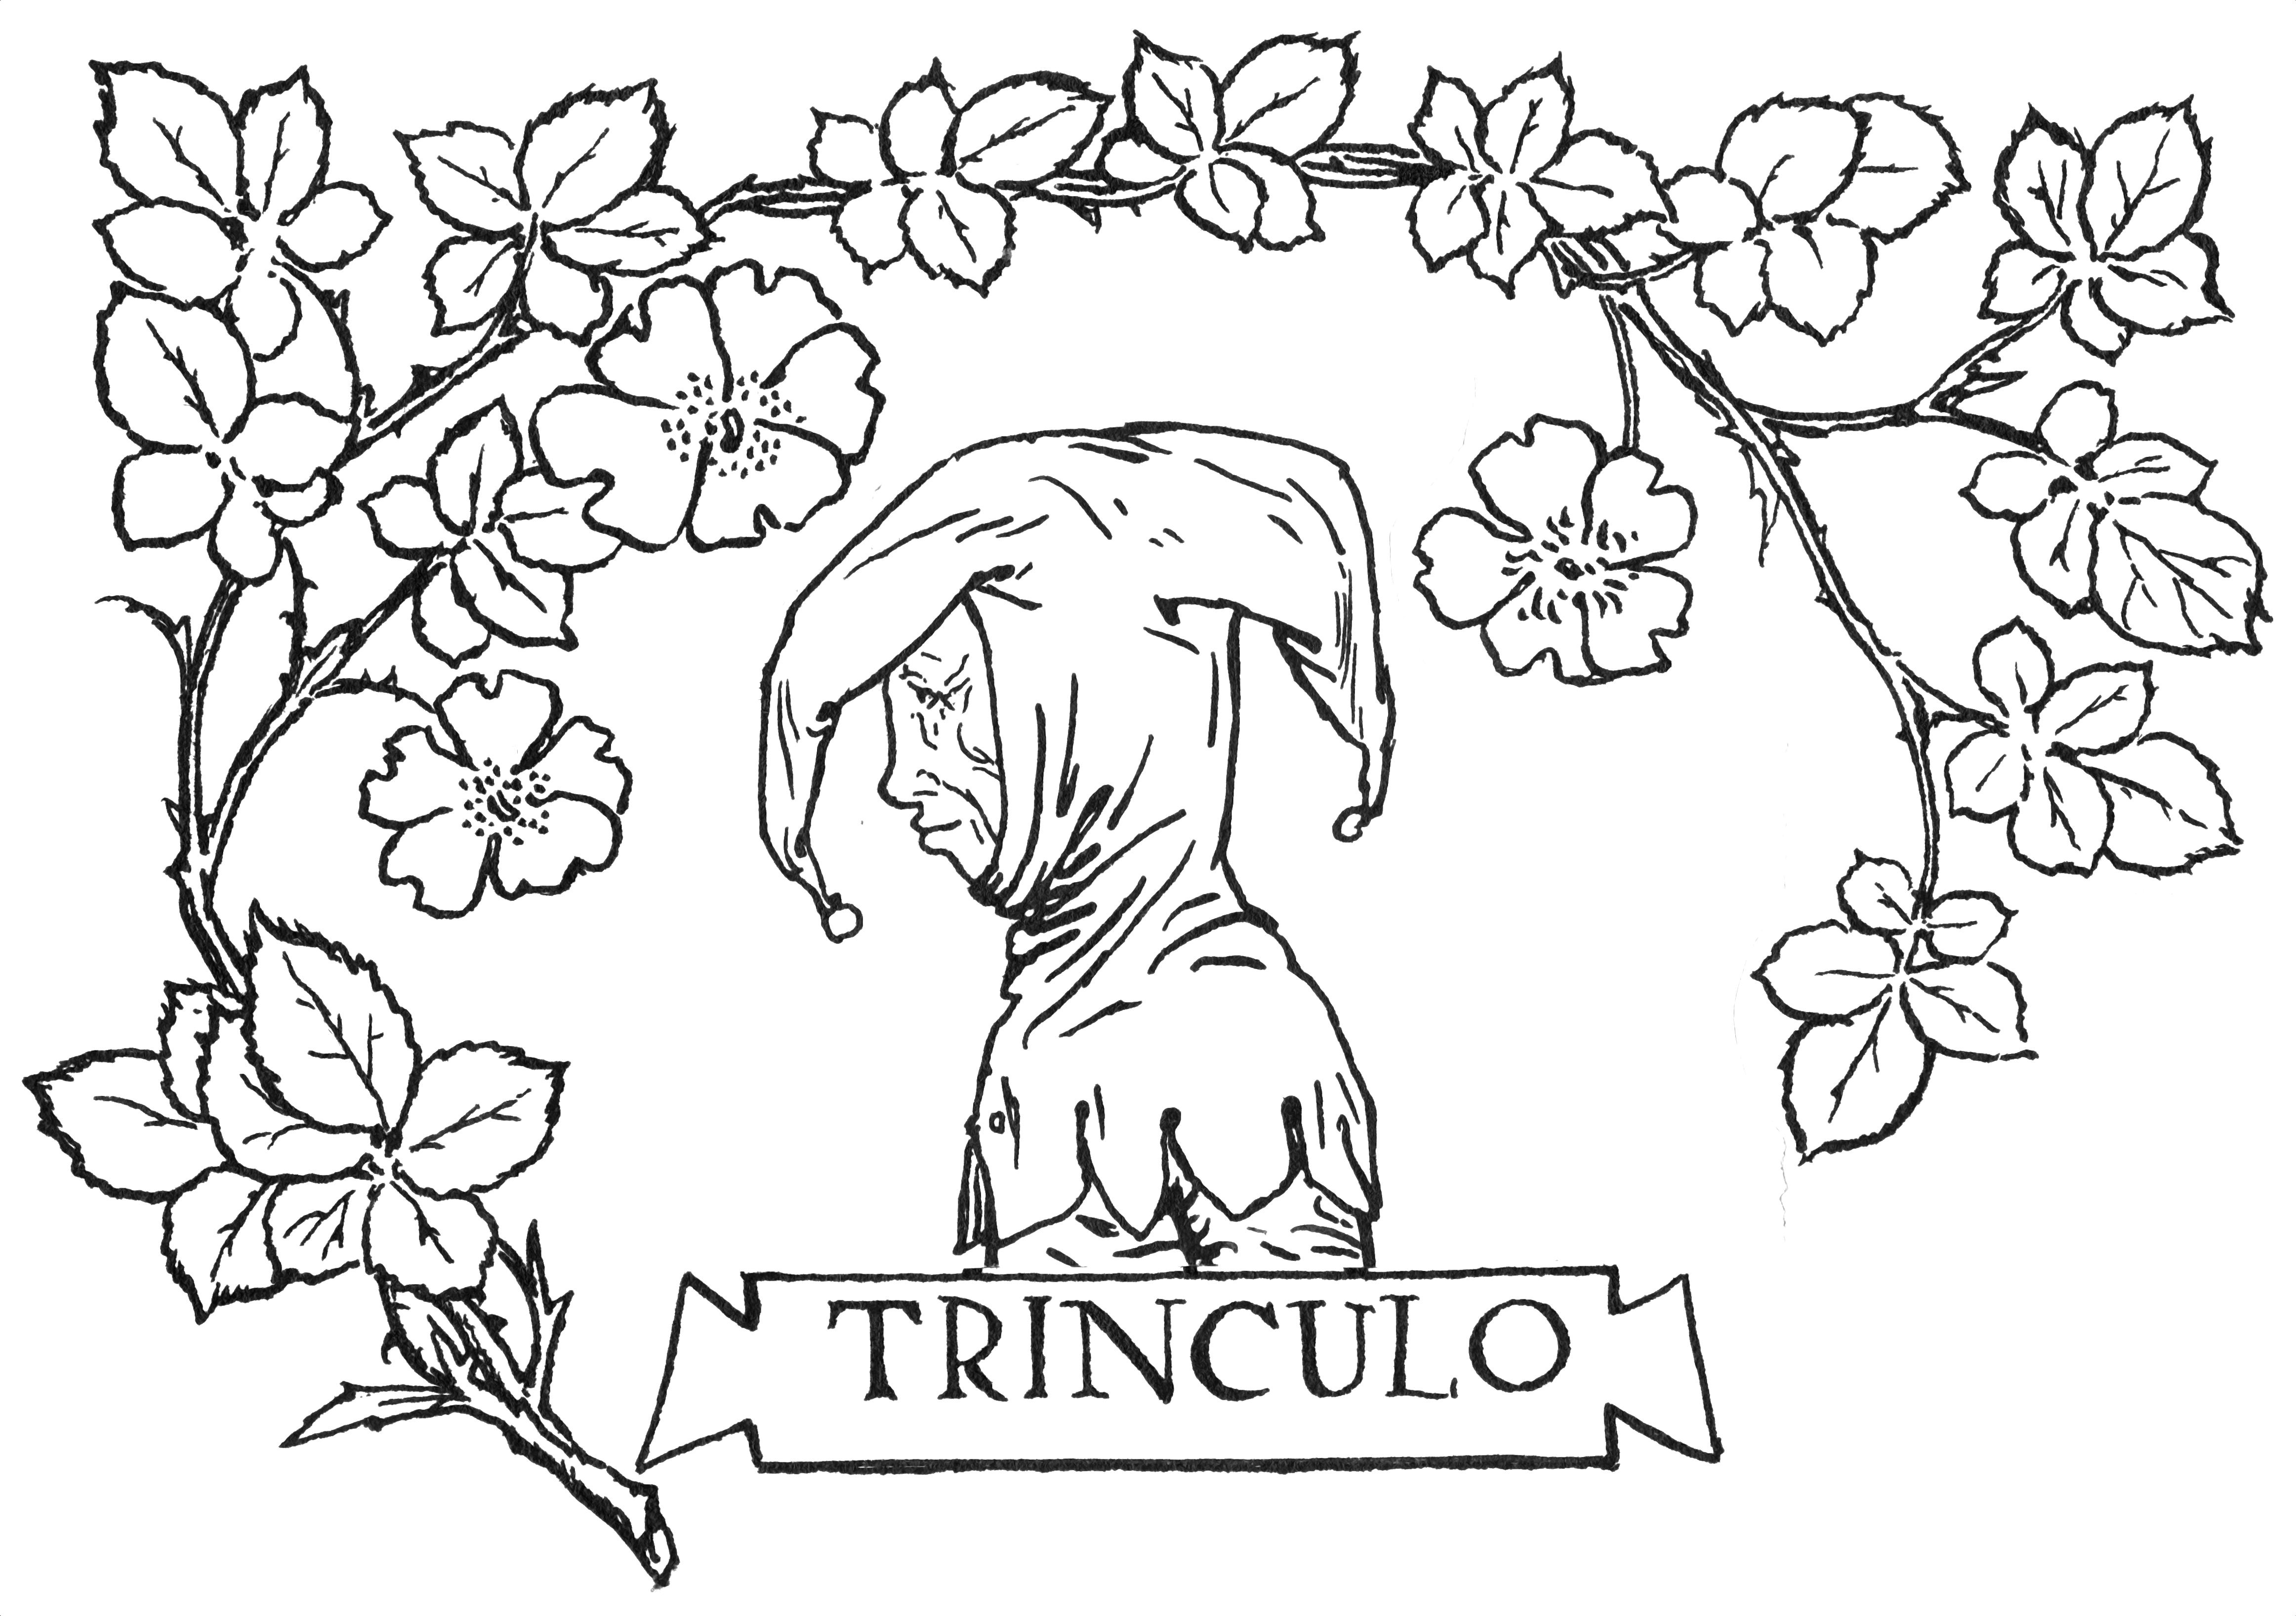
\includegraphics[width=\headerwidth]{2iiheadpiece}
\end{figure}

\enter{\textsc{Caliban} with a burden of wood. A noise of thunder heard.}

\begin{verse_speech}[Caliban] 
All the infections that the sun sucks up\\
From bogs, fens, flats, on Prosper fall and make him\\
By inch-meal a disease! His spirits hear me\\
And yet I needs must curse. But they'll nor pinch,\\
Fright me with urchin—shows, pitch me i' the mire,\\
Nor lead me, like a firebrand, in the dark\\
Out of my way, unless he bid 'em; but\\
For every trifle are they set upon me;\\
Sometime like apes that mow and chatter at me\\
And after bite me, then like hedgehogs which\\
Lie tumbling in my barefoot way and mount\\
Their pricks at my footfall; sometime am I\\
All wound with adders who with cloven tongues\\
Do hiss me into madness.

\enter{\textsc{Trinculo}}

Lo, now, lo!\\
Here comes a spirit of his, and to torment me\\
For bringing wood in slowly. I'll fall flat;\\
Perchance he will not mind me.
\end{verse_speech}

\begin{prose_speech}[Trinculo] 
Here's neither bush nor shrub, to bear off any weather at all, and another storm brewing; I hear it sing i' the wind: yond same black cloud, yond huge one, looks like a foul bombard that would shed his liquor. If it should thunder as it did before, I know not where to hide my head: yond same cloud cannot choose but fall by pailfuls. What have we here? a man or a fish? dead or alive? A fish: he smells like a fish; a very ancient and fish-like smell; a kind of not of the newest Poor-John. A strange fish! Were I in England now, as once I was, and had but this fish painted, not a holiday fool there but would give a piece of silver: there would this monster make a man; any strange beast there makes a man: when they will not give a doit to relieve a lame beggar, they will lazy out ten to see a dead Indian. Legged like a man and his fins like arms! Warm o' my troth! I do now let loose my opinion; hold it no longer: this is no fish, but an islander, that hath lately suffered by a thunderbolt.

\stage{Thunder.}

Alas, the storm is come again! my best way is to creep under his gaberdine; there is no other shelter hereabouts: misery acquaints a man with strange bed-fellows. I will here shroud till the dregs of the storm be past.
\end{prose_speech}

\begin{letter}
	\begin{figure}[tb]
		\centering
		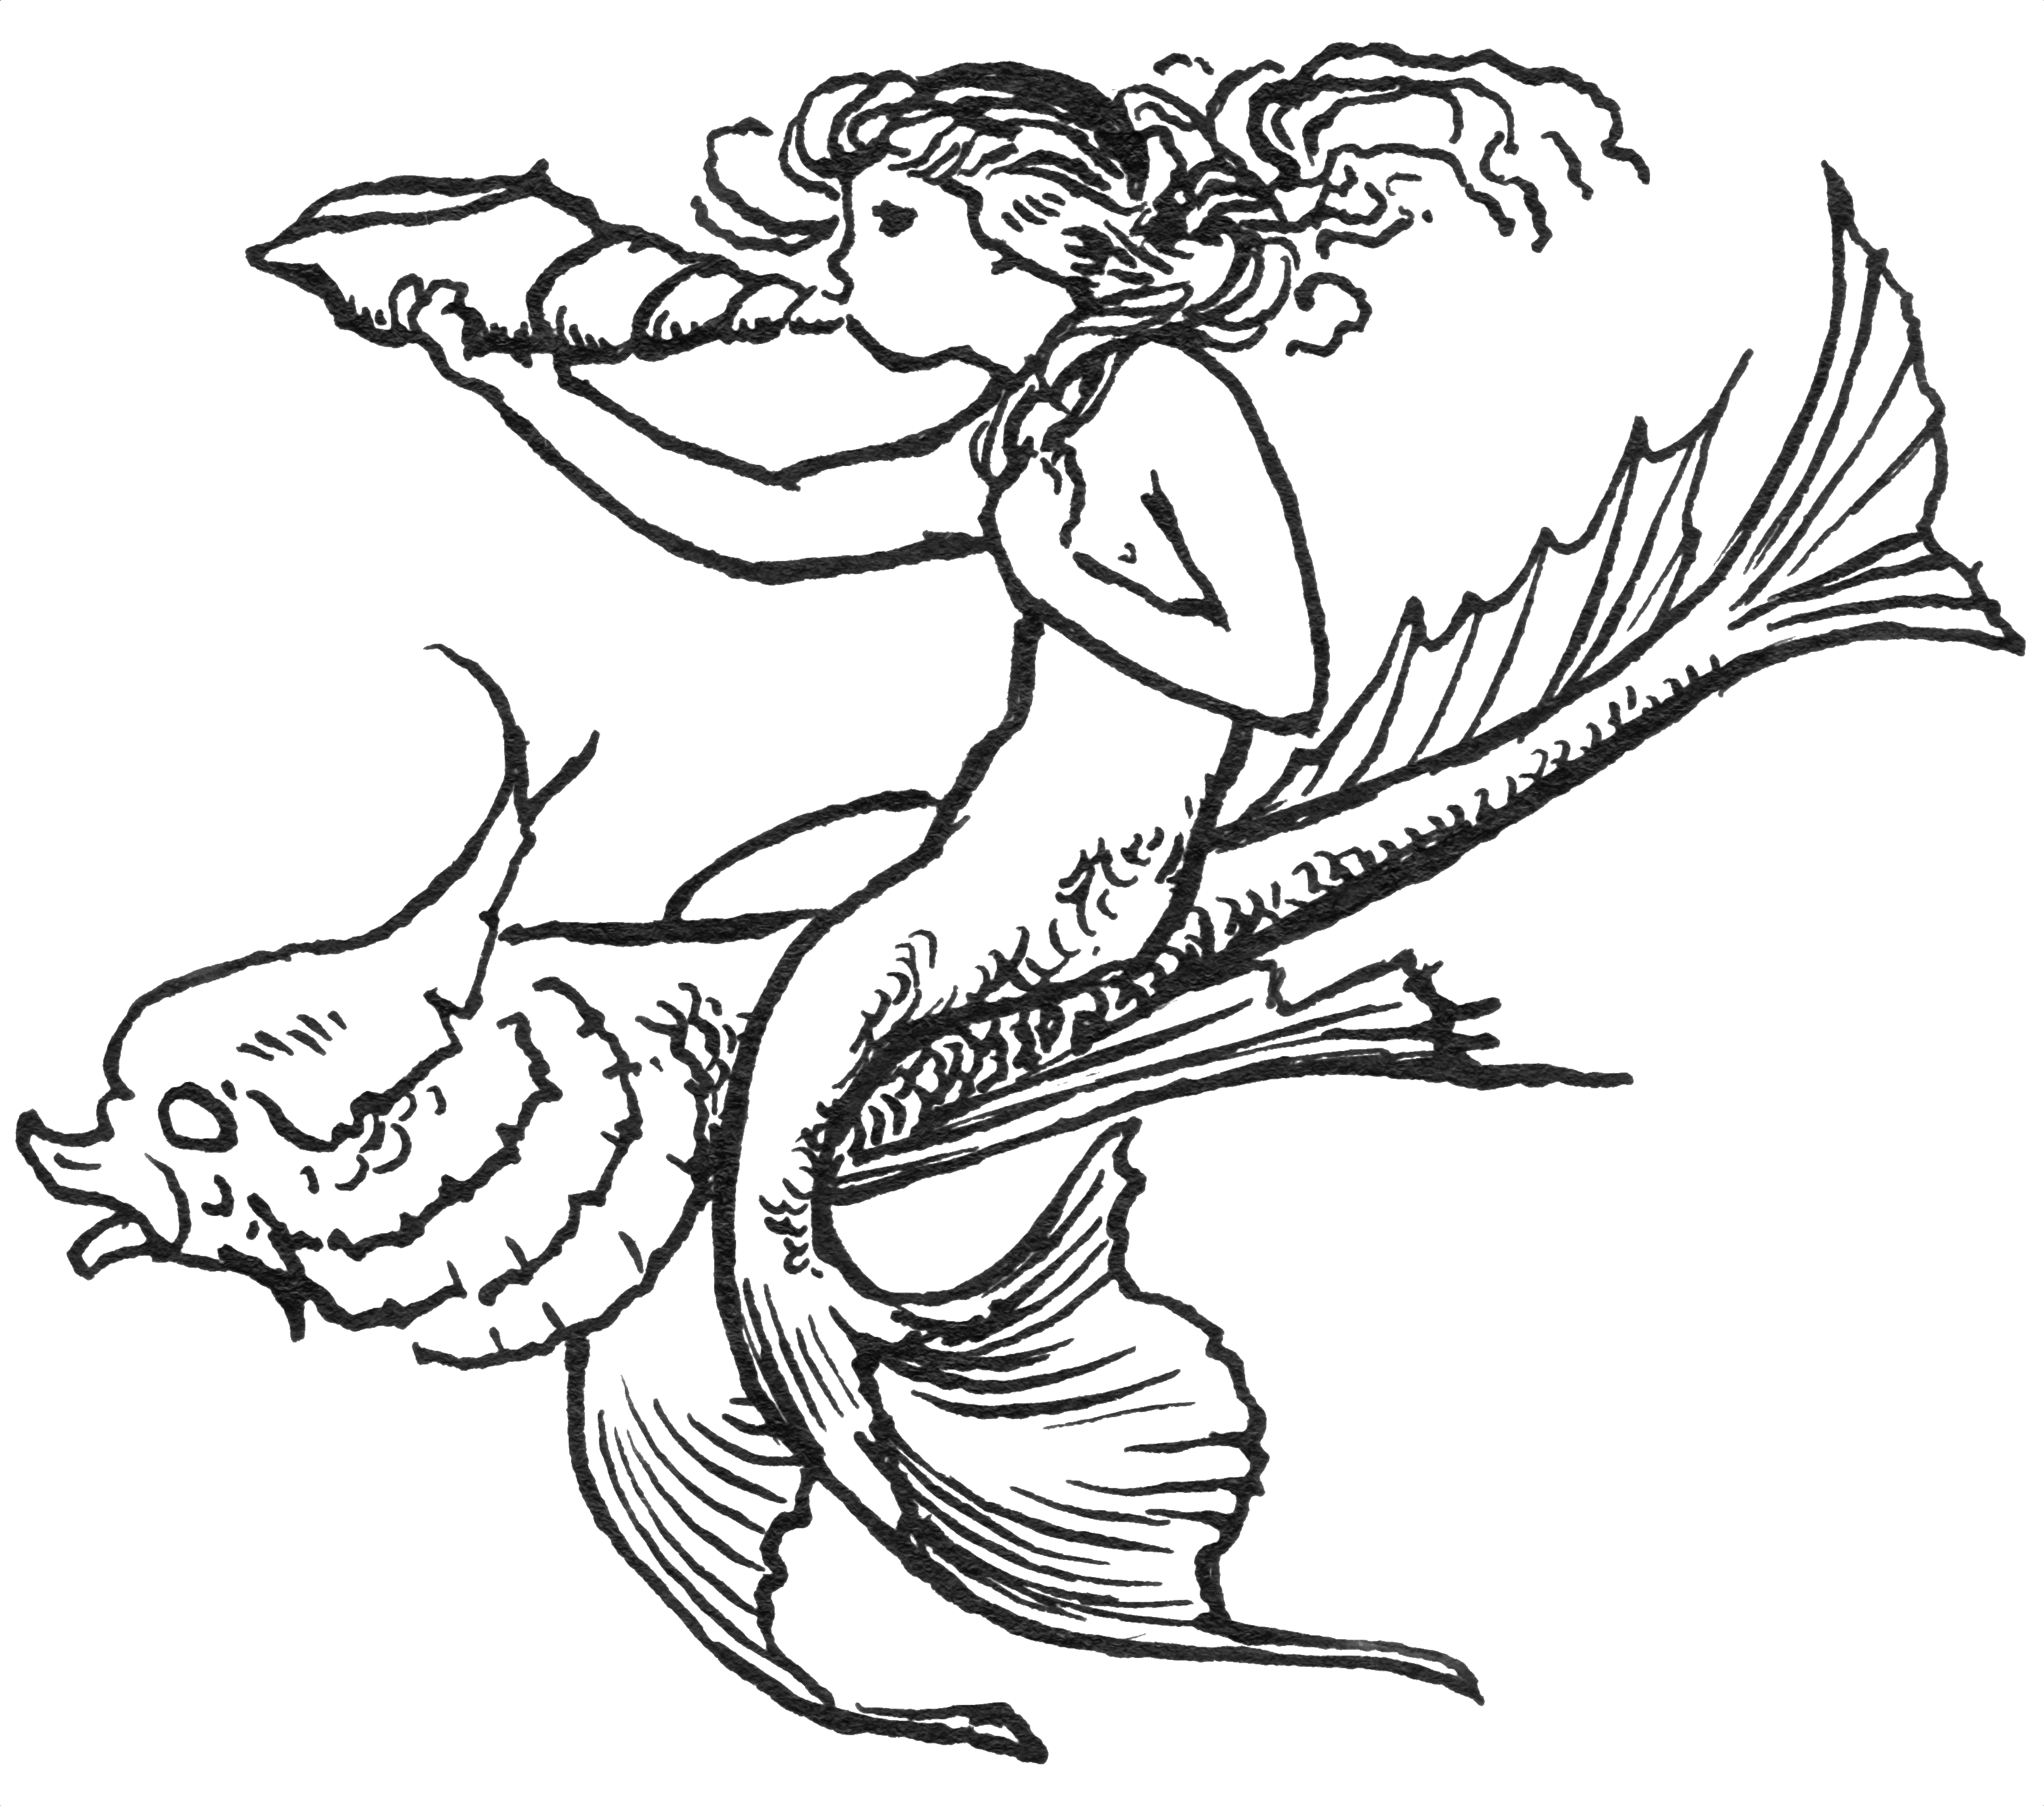
\includegraphics[width=.5\textwidth]{2iimerfish}
	\end{figure}
\end{letter}
\begin{a4}
	\begin{figure}[tb]
		\centering
		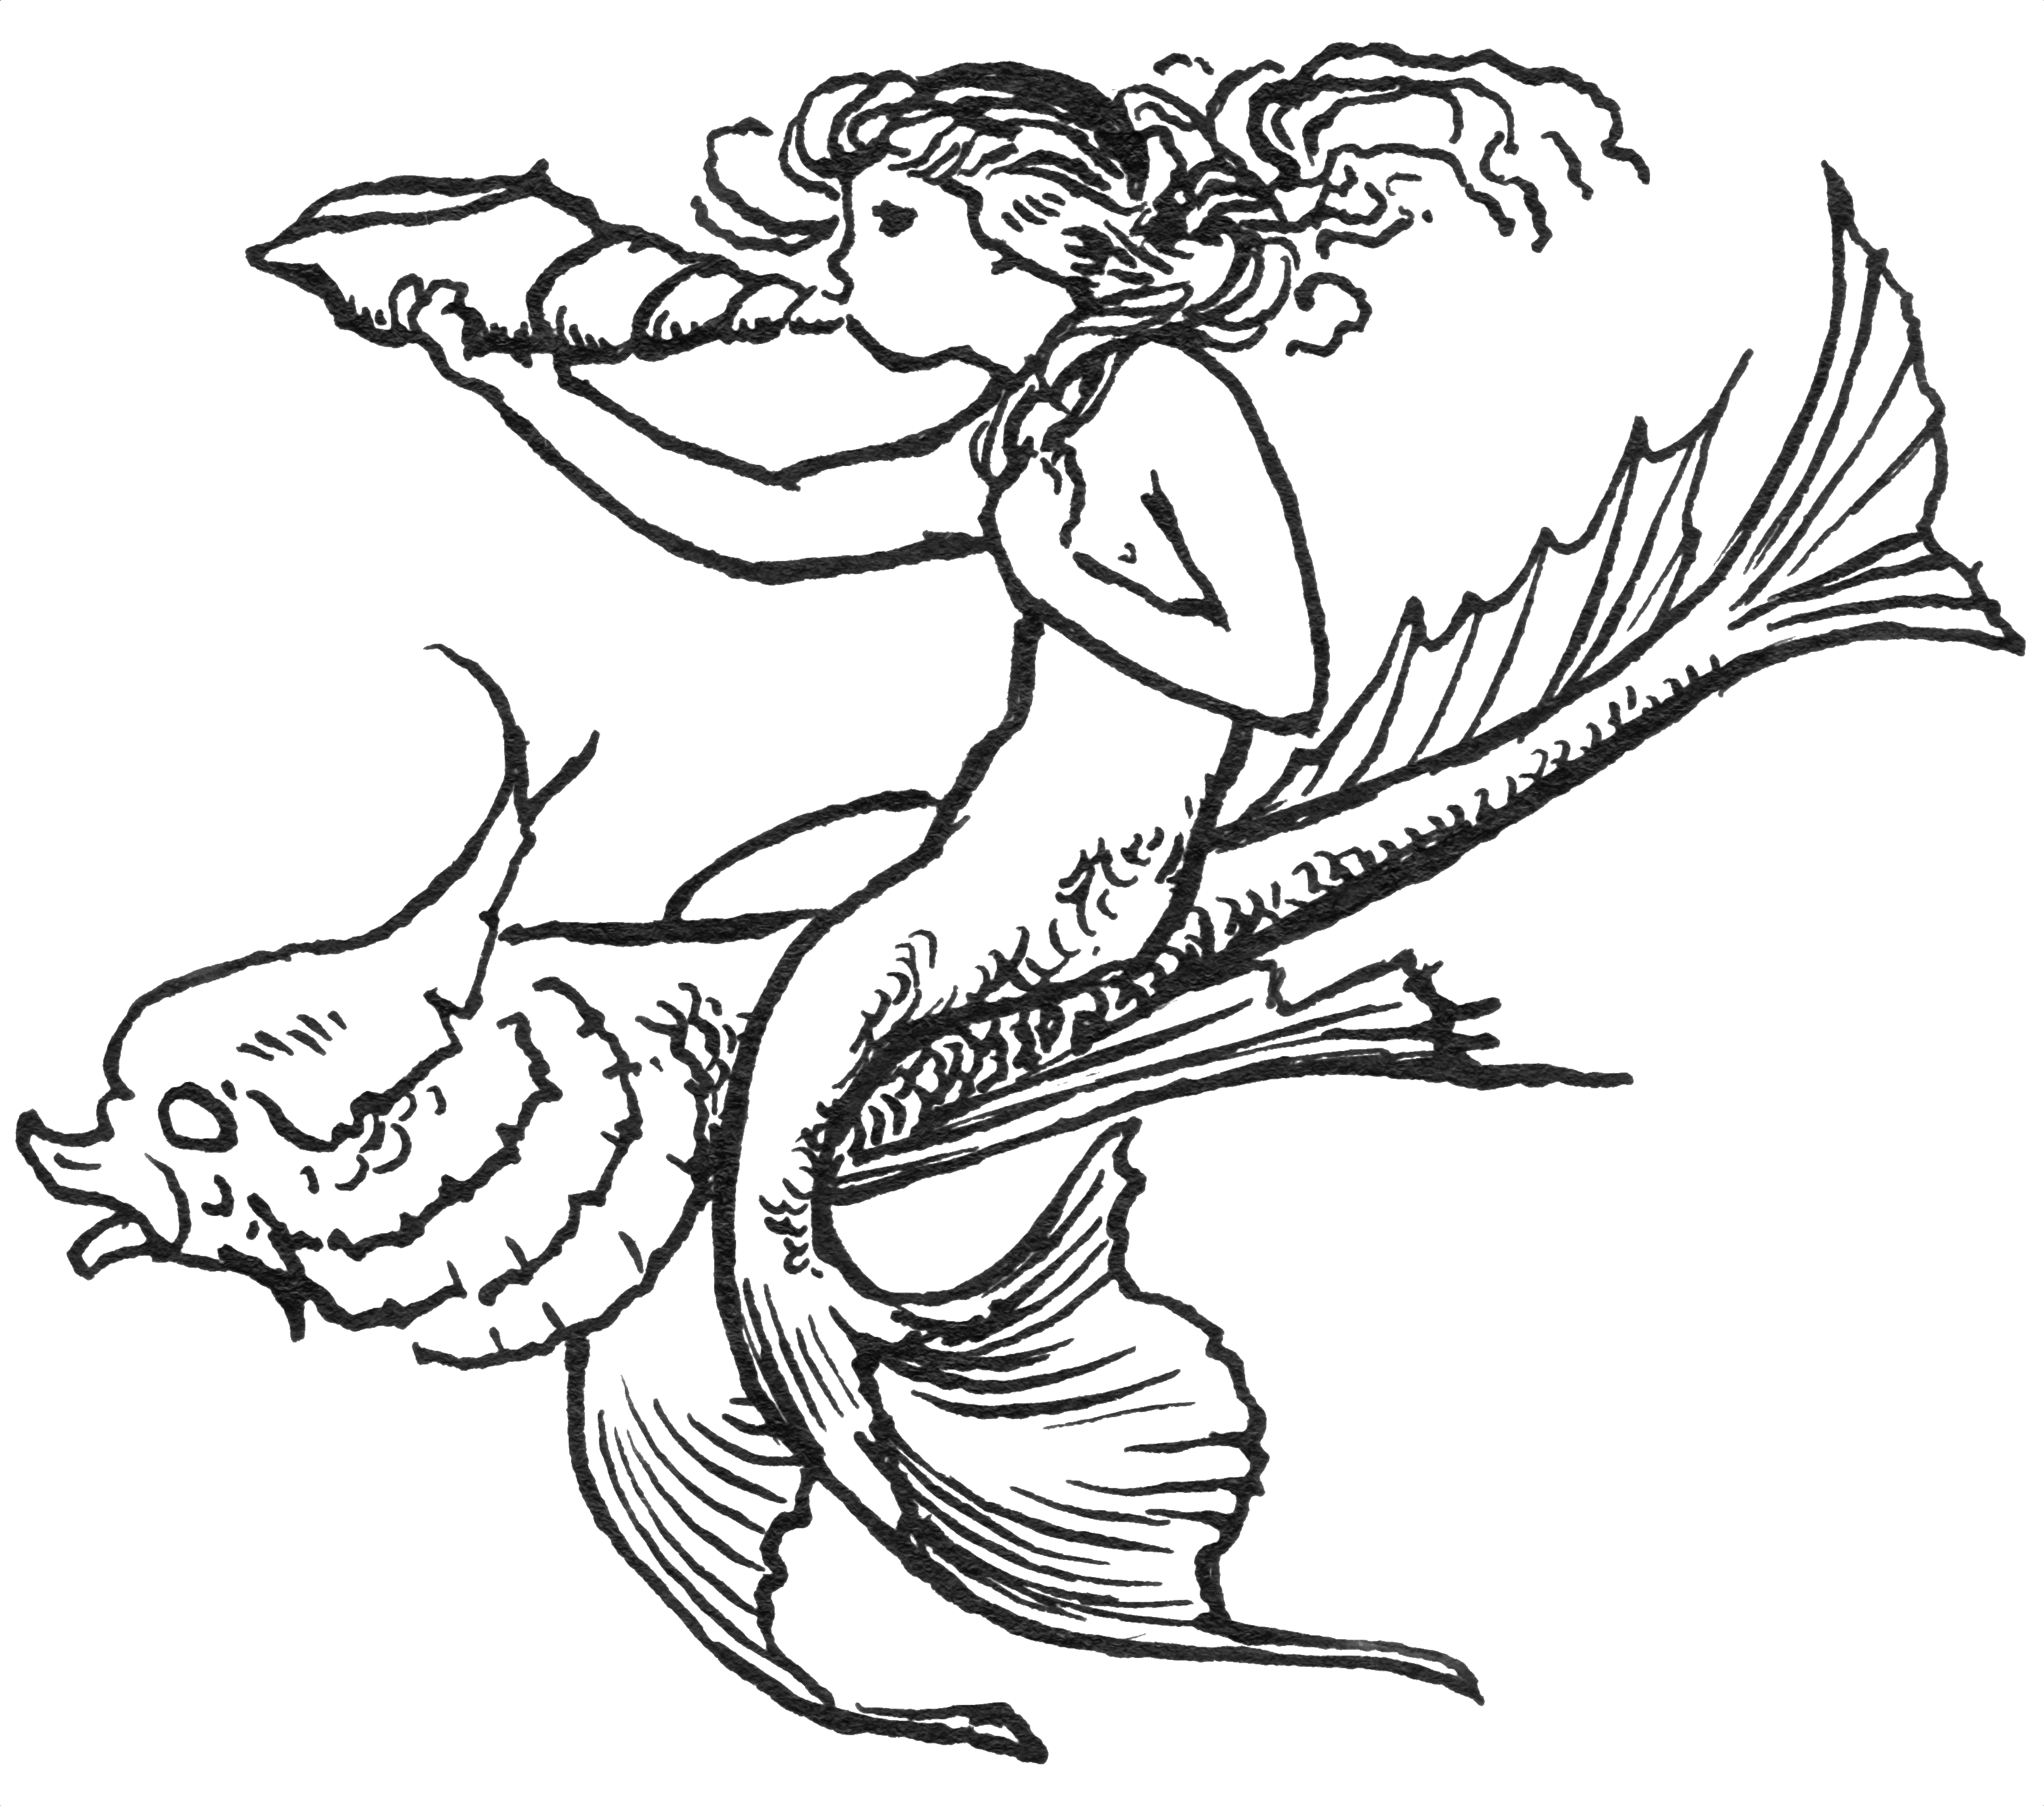
\includegraphics[width=.4\textwidth]{2iimerfish}
	\end{figure}
\end{a4}

\enter{\textsc{Stephano}, singing: a bottle in his hand}

\begin{prose_speech}[Stephano] 
\begin{song}
	\songline{I shall no more to sea, to sea,}
	\songline{Here shall I die ashore—}
\end{song}
This is a very scurvy tune to sing at a man's funeral: well, here's my comfort. \stage{Drinks}

\stage{Sings}

\begin{song}
	\songline{The master, the swabber, the boatswain and I,}
	\songline{The gunner and his mate}
	\songline{Loved Mall, Meg and Marian and Margery,}
	\songline{But none of us cared for Kate;}
	\songline{For she had a tongue with a tang,}
	\songline{Would cry to a sailor, Go hang!}
	\songline{She loved not the savour of tar nor of pitch,}
	\songline{Yet a tailor might scratch her where'er she did itch:}
	\songline{Then to sea, boys, and let her go hang!}
\end{song}

This is a scurvy tune too: but here's my comfort.
\stage{Drinks}
\end{prose_speech}

\begin{letter}
	\begin{figure}[tb]
		\centering
		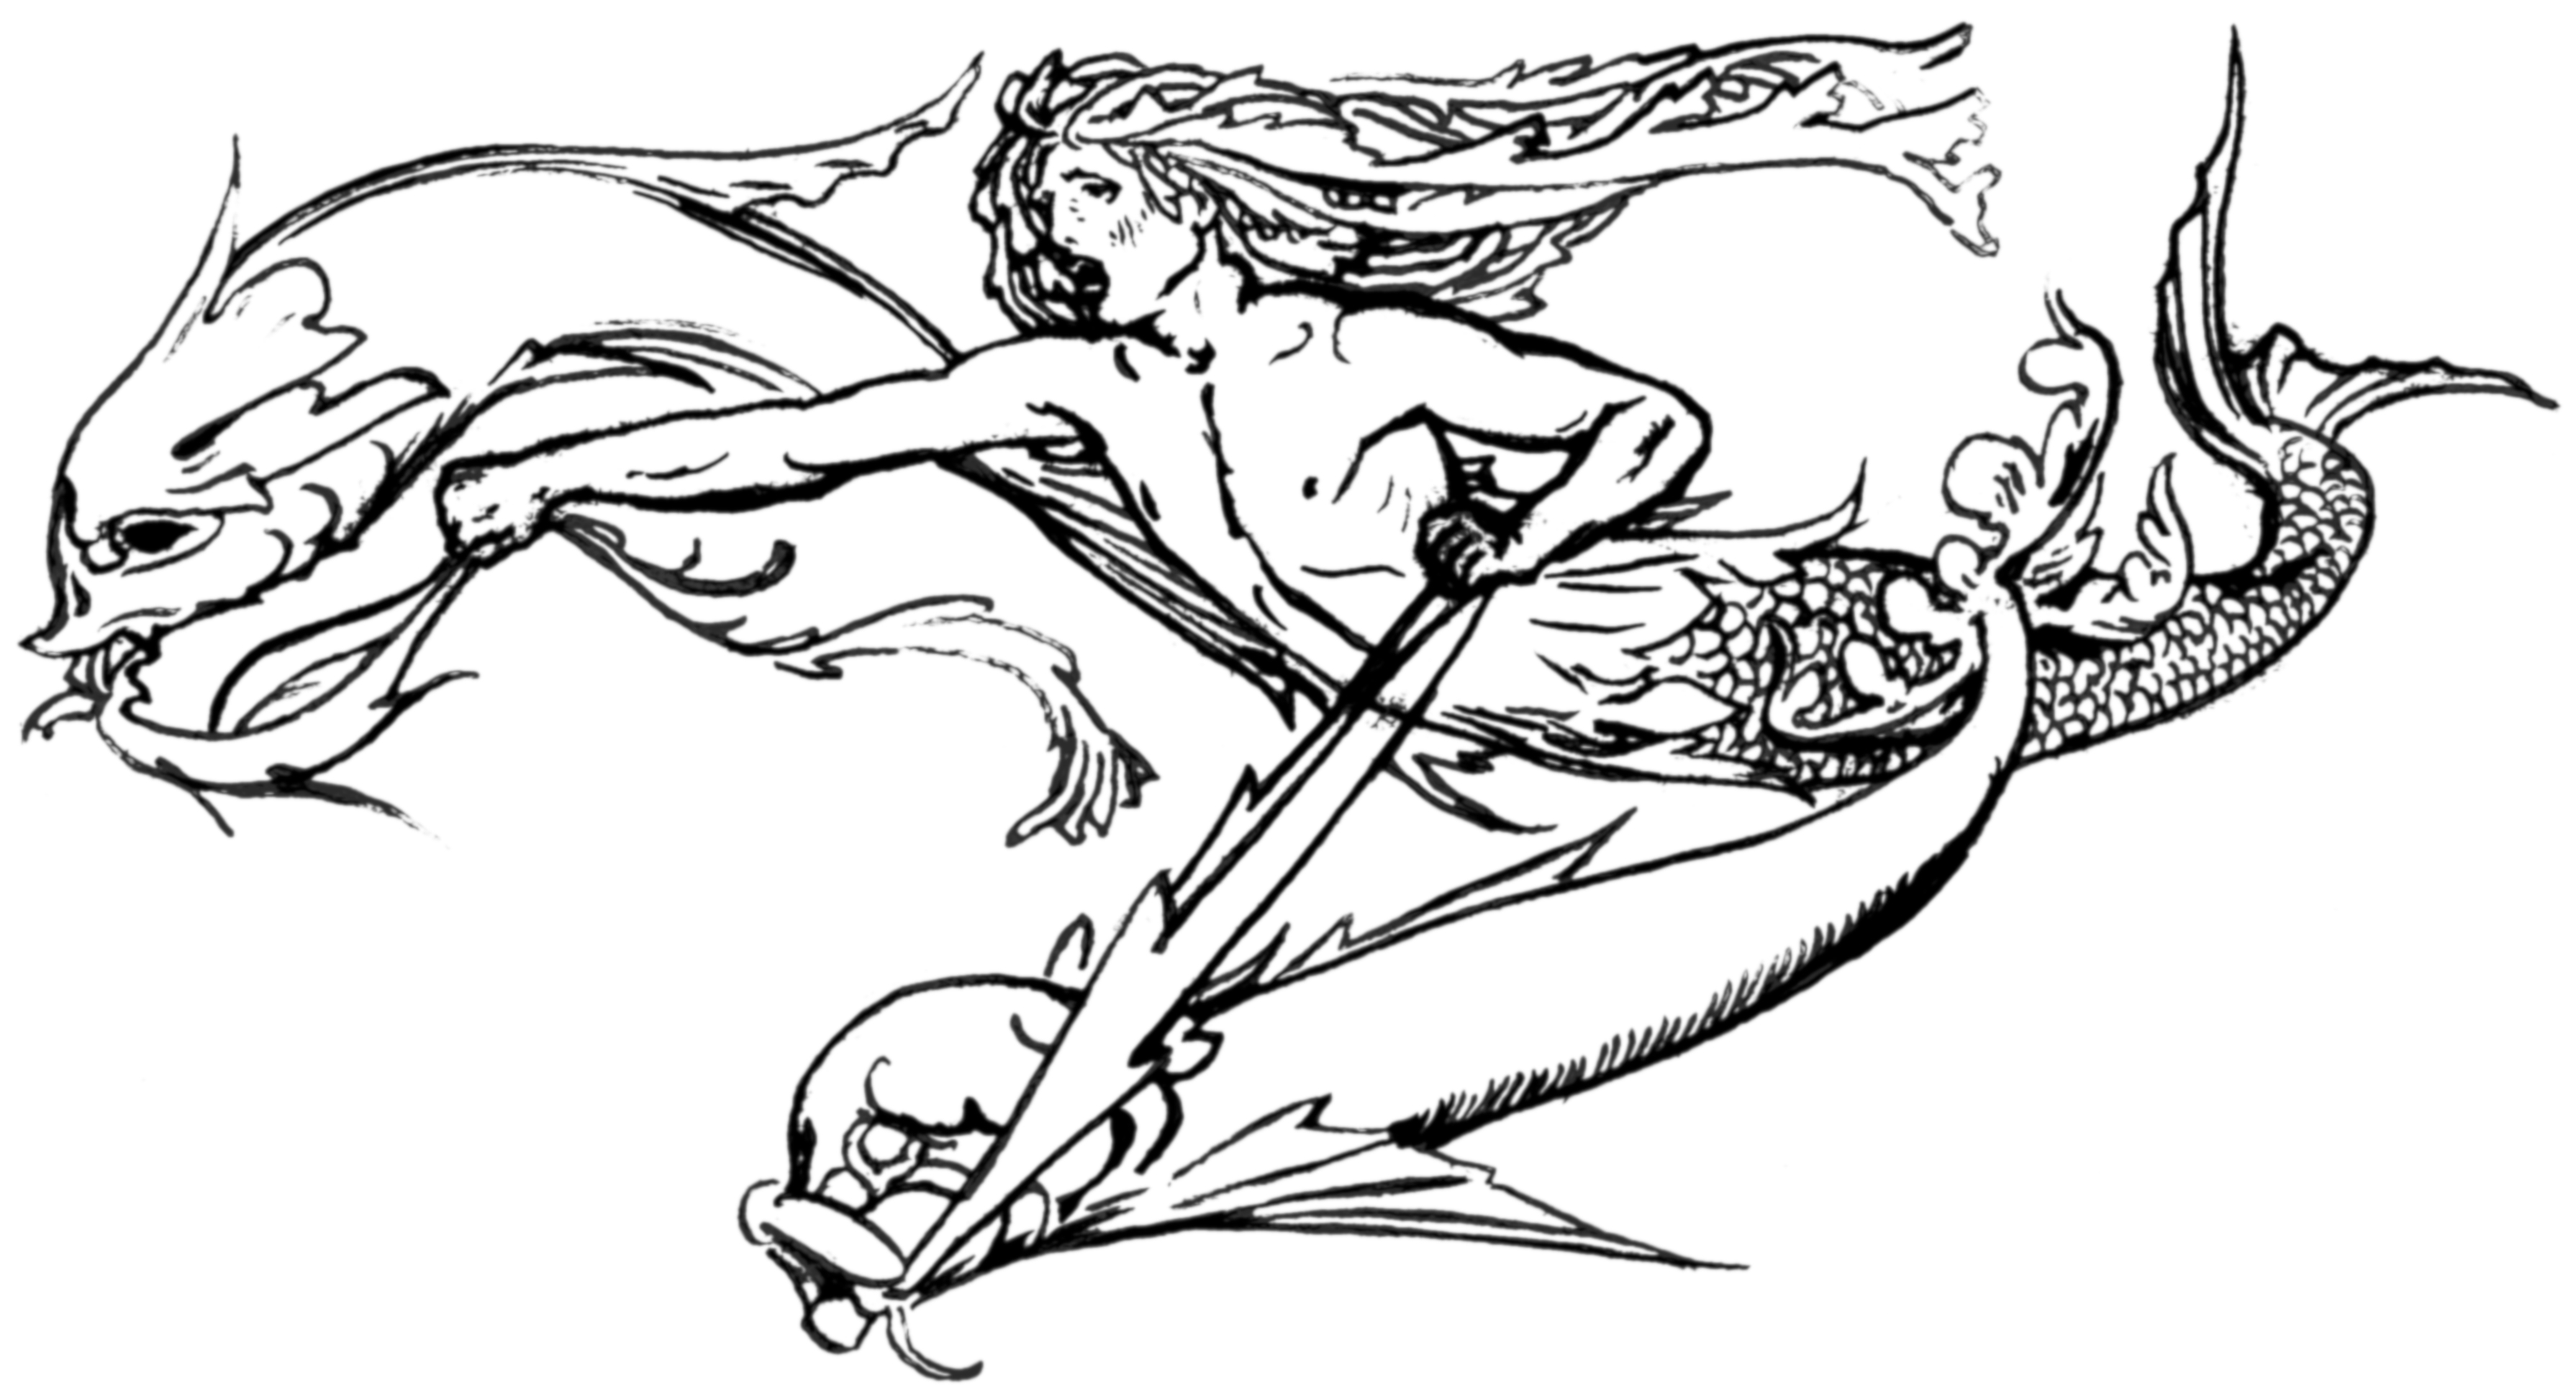
\includegraphics[width=\headerwidth]{2iifish}
	\end{figure}
\end{letter}

\begin{a4}
	\begin{figure}[tb]
		\centering
		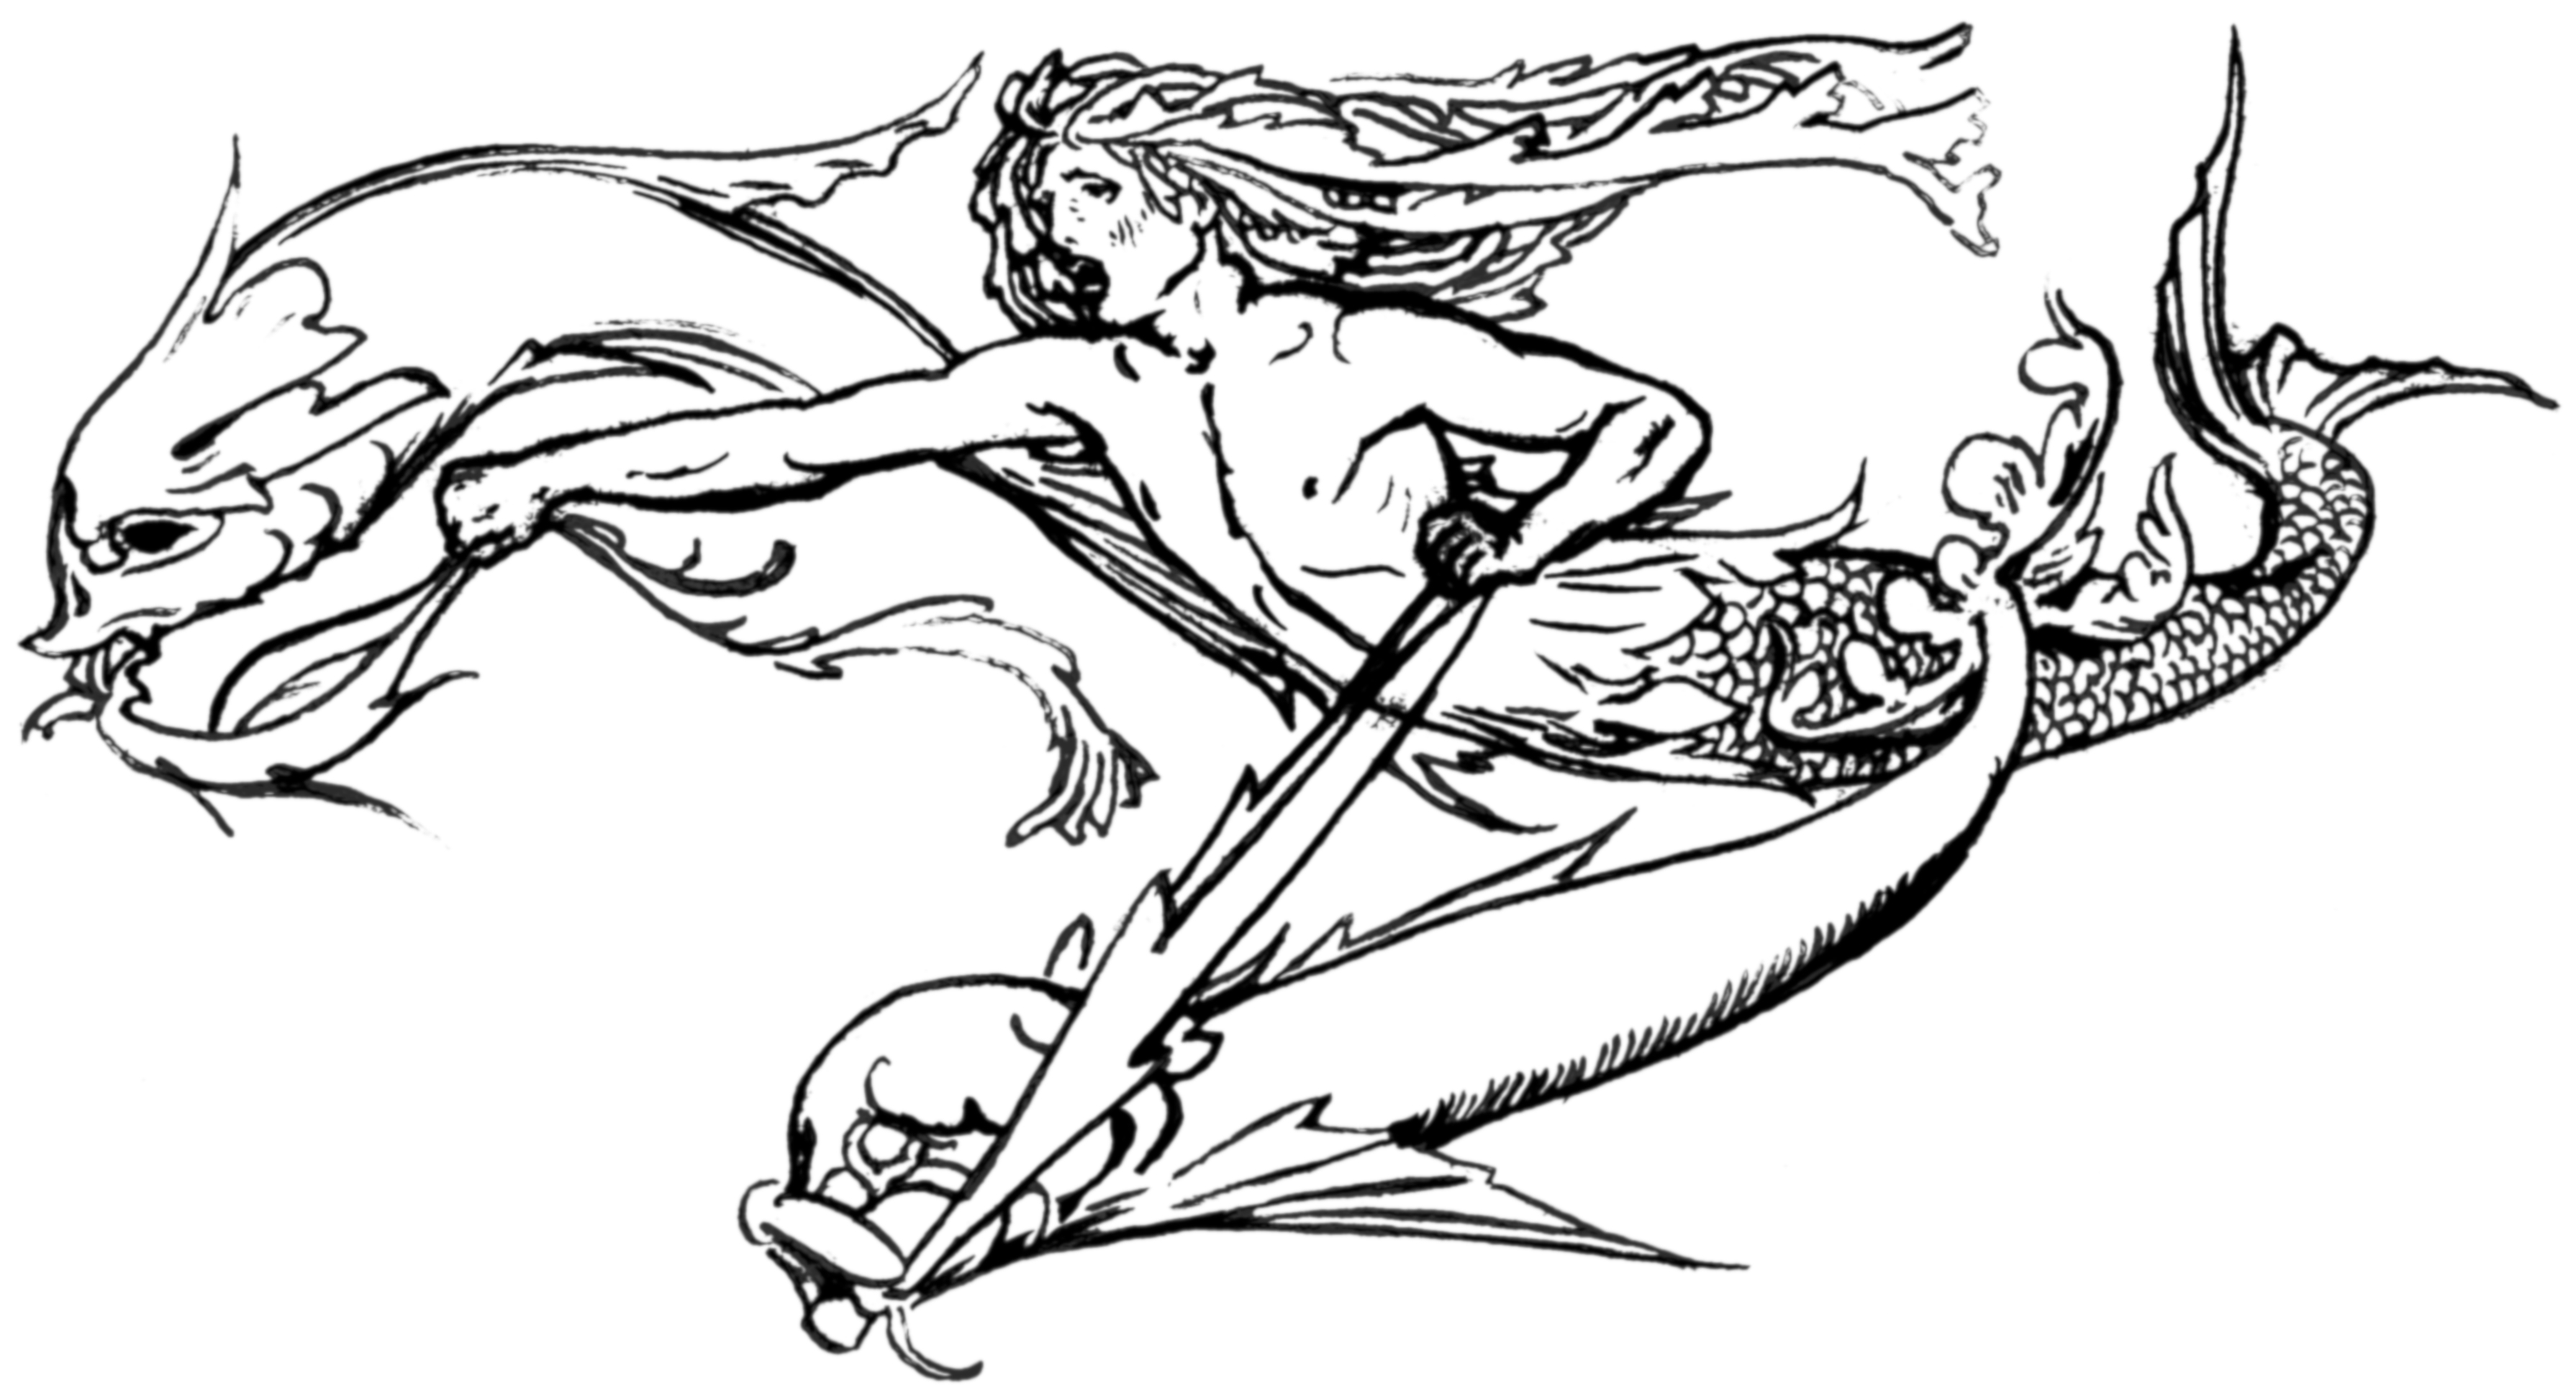
\includegraphics[width=.7\textwidth]{2iifish}
	\end{figure}
\end{a4}

\verseline[Caliban]{Do not torment me: Oh!} 
	
\begin{prose_speech}[Stephano] What's the matter? Have we devils here? Do you put tricks upon's with savages and men of Ind, ha? I have not scaped drowning to be afeard now of your four legs; for it hath been said, As proper a man as ever went on four legs cannot make him give ground; and it shall be said so again while Stephano breathes at's nostrils.
\end{prose_speech}


\verseline[Caliban]{The spirit torments me; Oh!} 

\begin{prose_speech}[Stephano] 
This is some monster of the isle with four legs, who hath got, as I take it, an ague. Where the devil should he learn our language? I will give him some relief, if it be but for that. if I can recover him and keep him tame and get to Naples with him, he's a present for any emperor that ever trod on neat's leather.
\end{prose_speech}


\verseline[Caliban]{Do not torment me, prithee; I'll bring my wood home faster.} 

\begin{prose_speech}[Stephano] 
He's in his fit now and does not talk after the wisest. He shall taste of my bottle: if he have never drunk wine afore will go near to remove his fit. If I can recover him and keep him tame, I will not take too much for him; he shall pay for him that hath him, and that soundly.
\end{prose_speech}

\begin{prose_speech}[Caliban] 
Thou dost me yet but little hurt; thou wilt anon, I know it by thy trembling: now Prosper works upon thee.
\end{prose_speech}

\begin{prose_speech}[Stephano] 
Come on your ways; open your mouth; here is that which will give language to you, cat: open your mouth; this will shake your shaking, I can tell you, and that soundly: you cannot tell who's your friend: open your chaps again.
\end{prose_speech}

\begin{prose_speech}[Trinculo] 
I should know that voice: it should be—but he is drowned; and these are devils: O defend me!
\end{prose_speech}

\begin{prose_speech}[Stephano] 
Four legs and two voices: a most delicate monster! His forward voice now is to speak well of his friend; his backward voice is to utter foul speeches and to detract. If all the wine in my bottle will recover him, I will help his ague. Come. Amen! I will pour some in thy other mouth.
\end{prose_speech}

\verseline[Trinculo]{Stephano!}
	
\begin{prose_speech}[Stephano] 
Doth thy other mouth call me? Mercy, mercy! This is a devil, and no monster: I will leave him; I have no long spoon.
\end{prose_speech}

\begin{prose_speech}[Trinculo] 
Stephano! If thou beest Stephano, touch me and speak to me: for I am Trinculo—be not afeard—thy good friend Trinculo.
\end{prose_speech}

\begin{prose_speech}[Stephano] 
If thou beest Trinculo, come forth: I'll pull thee by the lesser legs: if any be Trinculo's legs, these are they. Thou art very Trinculo indeed! How camest thou to be the siege of this moon-calf? can he vent Trinculos?
\end{prose_speech}

\begin{prose_speech}[Trinculo] 
I took him to be killed with a thunder-stroke. But art thou not drowned, Stephano? I hope now thou art not drowned. Is the storm overblown? I hid me under the dead moon-calf's gaberdine for fear of the storm. And art thou living, Stephano? O Stephano, two Neapolitans 'scaped!
\end{prose_speech}

\verseline[Stephano]{Prithee, do not turn me about; my stomach is not constant.} 

\begin{prose_speech}[Caliban] \aside{These be fine things, an if they be not sprites. That's a brave god and bears celestial liquor. I will kneel to him.}
\end{prose_speech}

\begin{prose_speech}[Stephano] 
How didst thou 'scape? How camest thou hither? swear by this bottle how thou camest hither. I escaped upon a butt of sack which the sailors heaved o'erboard, by this bottle; which I made of the bark of a tree with mine own hands since I was cast ashore.
\end{prose_speech}

\begin{pictures} %Stephano escapes the shipwreck
	
\begin{bwbigpic}
	[\picwidth]
	{2iibarrel}
	{}
\end{bwbigpic}

\end{pictures}

\verseline[Caliban]{I'll swear upon that bottle to be thy true subject; for the liquor is not earthly.} 

\verseline[Stephano]{Here; swear then how thou escapedst.} 

\verseline[Trinculo]{Swum ashore. man, like a duck: I can swim like a duck, I'll be sworn.} 

\verseline[Stephano]{Here, kiss the book. Though thou canst swim like a duck, thou art made like a goose.} 

\verseline[Trinculo]{O Stephano. hast any more of this?} 

\verseline[Stephano]{The whole butt, man: my cellar is in a rock by the sea-side where my wine is hid. How now, moon-calf! how does thine ague?} 

\verseline[Caliban]{Hast thou not dropp'd from heaven?} 

\verseline[Stephano]{Out o' the moon, I do assure thee: I was the man i' the moon when time was.} 

\verseline[Caliban]{I have seen thee in her and I do adore thee: my mistress show'd me thee and thy dog and thy bush.} 

\verseline[Stephano]{Come, swear to that; kiss the book: I will furnish it anon with new contents swear.} 

\begin{prose_speech}[Trinculo] 
By this good light, this is a very shallow monster! I afeard of him! A very weak monster! The man i' the moon! A most poor credulous monster! Well drawn, monster, in good sooth!
\end{prose_speech}

\verseline[Caliban]{I'll show thee every fertile inch o' th' island; and I will kiss thy foot: I prithee, be my god.} 

\verseline[Trinculo]{By this light, a most perfidious and drunken monster! when 's god's asleep, he'll rob his bottle.} 

\verseline[Caliban]{I'll kiss thy foot; I'll swear myself thy subject.} 

\verseline[Stephano]{Come on then; down, and swear.} 

\verseline[Trinculo]{I shall laugh myself to death at this puppy-headed monster. A most scurvy monster! I could find in my heart to beat him,—} 

\verseline[Stephano]{Come, kiss.} 

\verseline[Trinculo]{But that the poor monster's in drink: an abominable monster!} 


\begin{pictures} %Caliban celebrates - a4
	\begin{a4}
		\begin{bwbigpic}
			[\picwidth]
			{2iinewmaster}
			{}
		\end{bwbigpic}
	\end{a4}
\end{pictures}

\begin{verse_speech}[Caliban] 
I'll show thee the best springs; I'll pluck thee berries;\\
I'll fish for thee and get thee wood enough.\\
A plague upon the tyrant that I serve!\\
I'll bear him no more sticks, but follow thee,\\
Thou wondrous man.
\end{verse_speech}

\begin{verse_speech}[Trinculo]
A most ridiculous monster, to make a wonder of a\\
Poor drunkard!
\end{verse_speech}

\begin{verse_speech}[Caliban] 
I prithee, let me bring thee where crabs grow;\\
And I with my long nails will dig thee pignuts;\\
Show thee a jay's nest and instruct thee how\\
To snare the nimble marmoset; I'll bring thee\\
To clustering filberts and sometimes I'll get thee\\
Young scamels from the rock. Wilt thou go with me?
\end{verse_speech}

\begin{prose_speech}[Stephano] 
I prithee now, lead the way without any more talking. Trinculo, the king and all our company else being drowned, we will inherit here: here; bear my bottle: fellow Trinculo, we'll fill him by and by again.
\end{prose_speech}

\begin{prose_speech}[Caliban] 
\stage{Sings drunkenly}
Farewell master; farewell, farewell!
\end{prose_speech}

\begin{pictures} %Caliban celebrates - letter
	\begin{letter}
		\begin{bwbigpic}
			[\picwidth]
			{2iinewmaster}
			{}
		\end{bwbigpic}
	\end{letter}
\end{pictures}

\verseline[Trinculo]{A howling monster: a drunken monster!} 

\begin{verse_speech}[Caliban] 
No more dams I'll make for fish\\
Nor fetch in firing\\
At requiring;\\
Nor scrape trencher, nor wash dish\\
'Ban, 'Ban, Cacaliban\\
Has a new master: get a new man.\\
Freedom, hey-day! hey-day, freedom! freedom,\\
hey-day, freedom!
\end{verse_speech}

\verseline[Stephano]{O brave monster! Lead the way.} 

\exeunt{}

\begin{letter}
	\vfill

	\begin{center}
		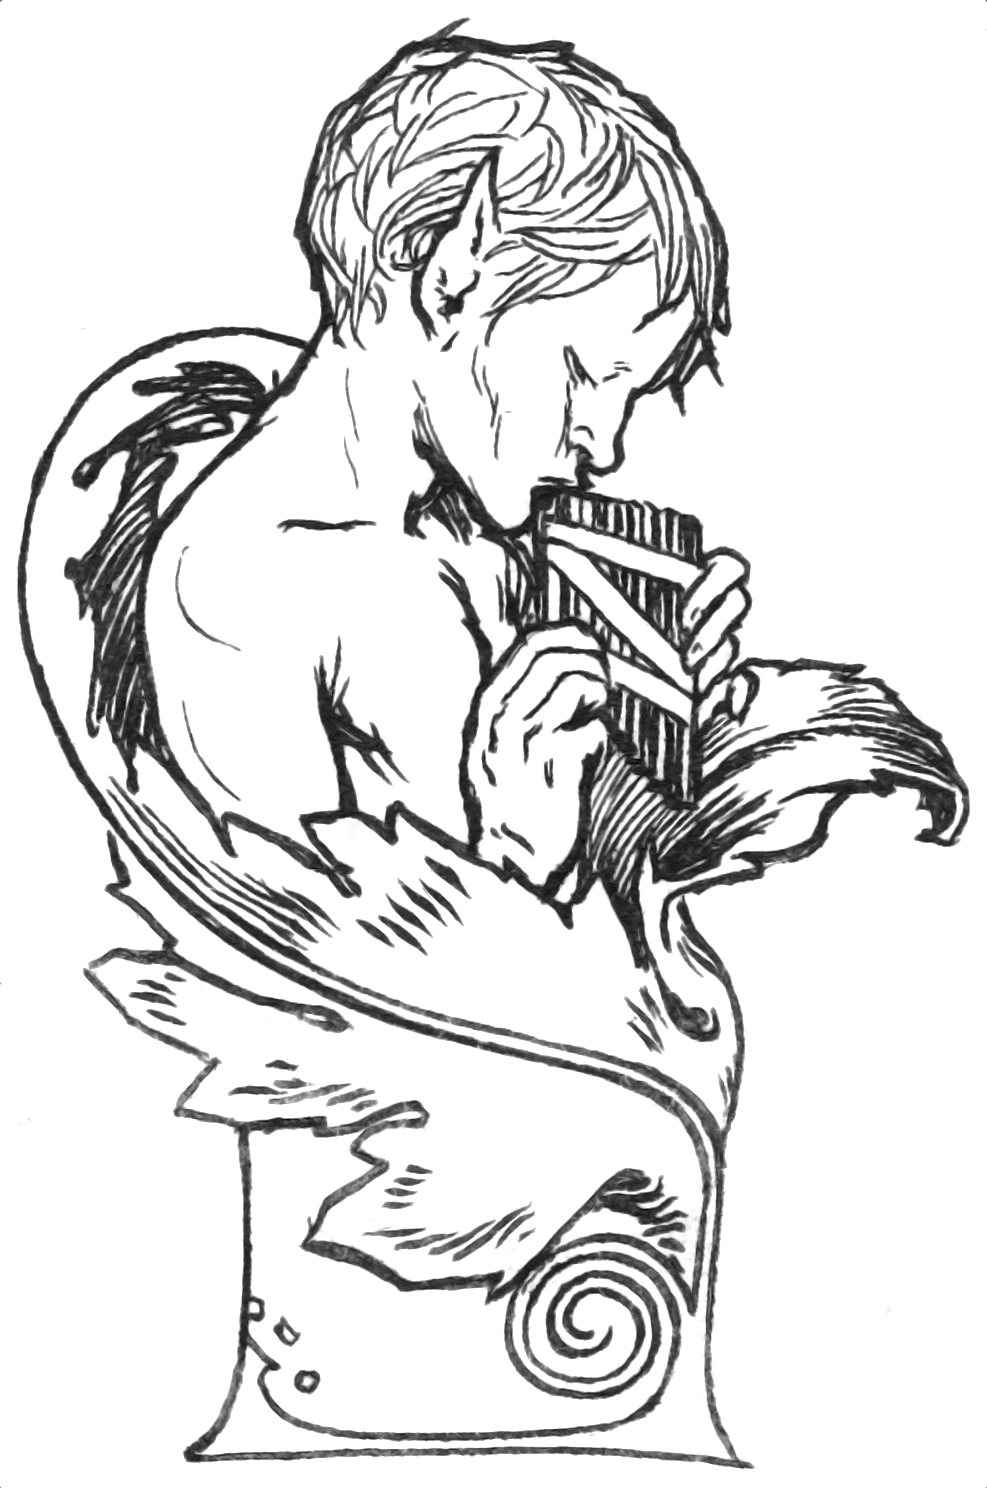
\includegraphics[width=.4\textwidth]{2iitailpiece}
	\end{center}
\end{letter}


\begin{a4}
	\begin{tikzpicture}[remember picture, overlay]
		\node (dropcap) at ($(current page.south)+(0cm,6cm)$) {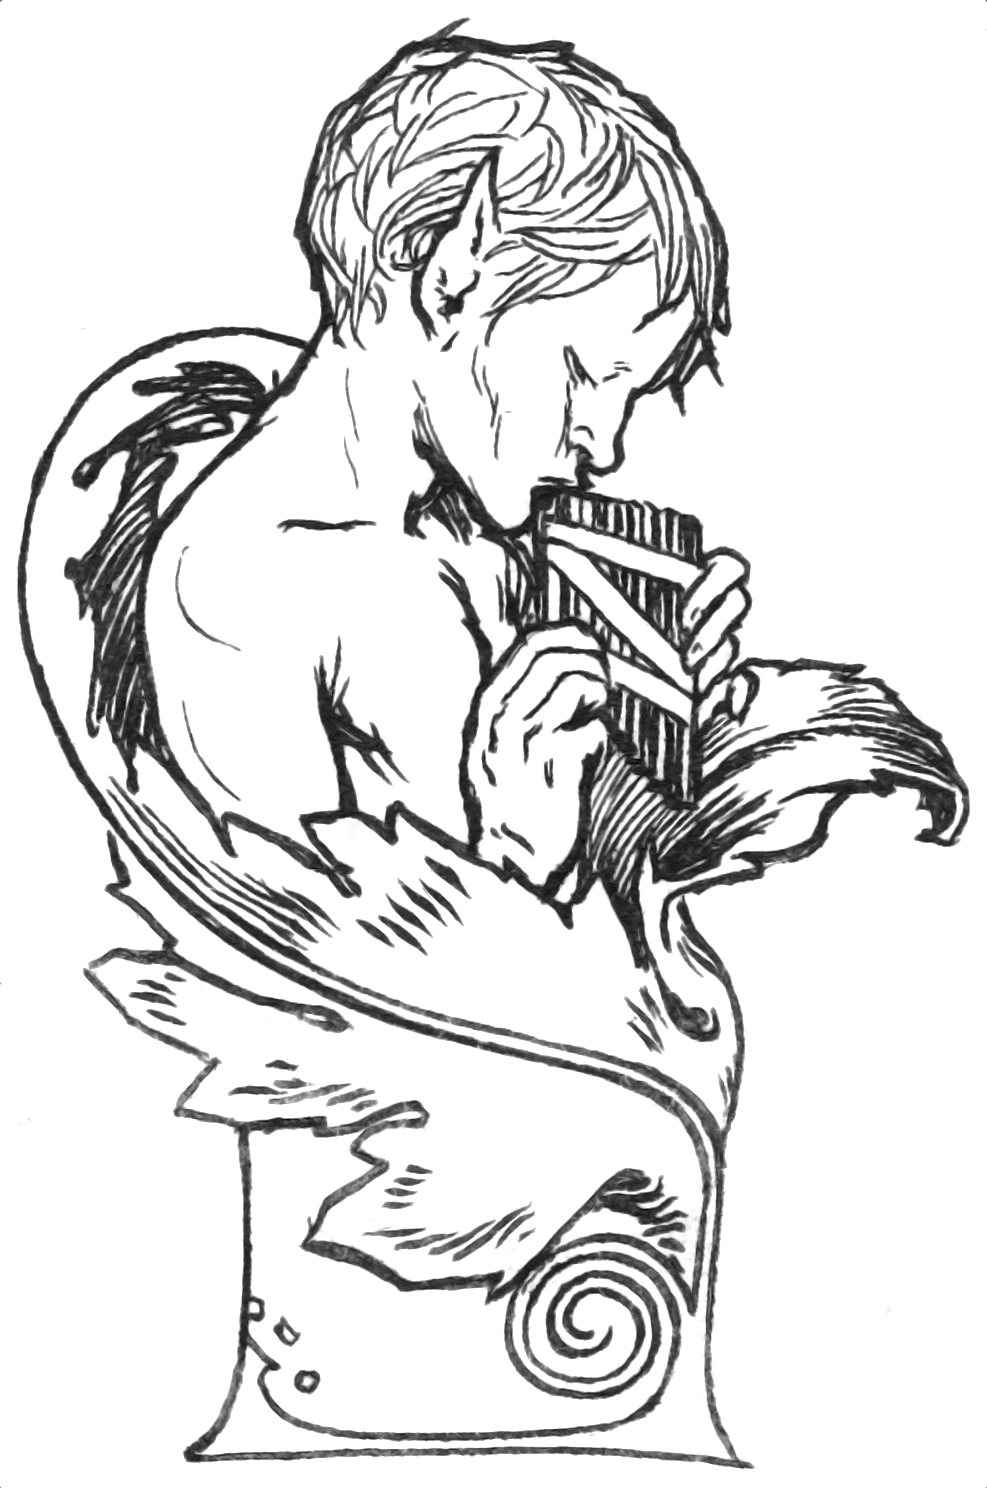
\includegraphics[width=.3\textwidth]{2iitailpiece}};
	\end{tikzpicture}
\end{a4}



